\subsection{Progettazione di dettaglio e codifica}
Questa fase comincia in seguito a quella precedente e termina con la \textit{Revisione di Qualifica}, ovvero dal x/x/x al x/x/x.\\
Di seguito vengono riportate tutte le attività.

\begin{itemize}
	\item \textbf{Incremento e verifica dei documenti}: verrà realizzato un documento contenente tutte le caratteristiche del prodotto e il cosiddetto \textit{Manuale utente}. Inoltre, in caso di necessità, alcuni documenti verranno aggiornati;
	\item \textbf{Incremento e verifica delle attività}: viene ampliato lo studio delle tecnologie mancanti, necessarie per lo sviluppo del prodotto; 
	\item \textbf{\glo{Product Baseline}}: vengono realizzati i \textit{diagrammi delle classi}, che consentono di descrivere tipi di entità (con le loro caratteristiche e le eventuali relazioni), e i \textit{diagrammi delle attività}, che permettono di descrivere i vari processi. Inoltre verranno analizzati design patterns esistenti, con il fine di scegliere quello più adatto per il prodotto da creare.
	\item \textbf{\glo{Scrittura del codice e incrementi}}: viene realizzata la codifica, partendo dal \textit{Proof of Concept} già presente. Gli incrementi consistono nell'implementare sempre più casi d'uso, stabiliti nell'\textit{Analisi dei Rischi}, iterando tra progettazione di dettaglio e realizzazione. La priorità sarà nei confronti di quelli obbligatori: in questo modo per ciascun caso d'uso, nell'eventualità di mancato completamento entro il periodo stabilito, è possibile attuare in sicurezza una ripianificazione dell'attività in questione. \textbf{qui andrebbero aggiunti i periodi in cui si fanno gli incrementi ovvero i blocchi di UC riportando il codice}
\end{itemize}

\subsubsection{Periodi}
La pianificazione di questa fase è stata organizzata nel modo seguente:
\textbf{riassunto della parte precedente, specificando quando di vanno a fare le cose}
\begin{itemize}
\item \textbf{xx/xx/2020 - xx/x/2020}: \textbf{sistemare i documenti e aver appreso le nuove tecnologie che mancavano da studiare}.

\item \textbf{xx/xx/2020 - xx/x/2020}: \textbf{aver finito il primo incremento ovvero il primo blocco di UC definiti prima nella codifica}.

\item \textbf{xx/xx/2020 - xx/x/2020}: \textbf{aver finito il secondo incremento ovvero il secondo blocco di UC definiti prima nella codifica}.

\item .......via così

\item \textbf{xx/xx/2020 - xx/xx/2020}: \textbf{stesura e verifica dei nuovi documenti}.
\end{itemize}

\subsubsection{Diagramma di Gantt: Progettazione di dettaglio e Codifica}
\begin{figure}[h]
	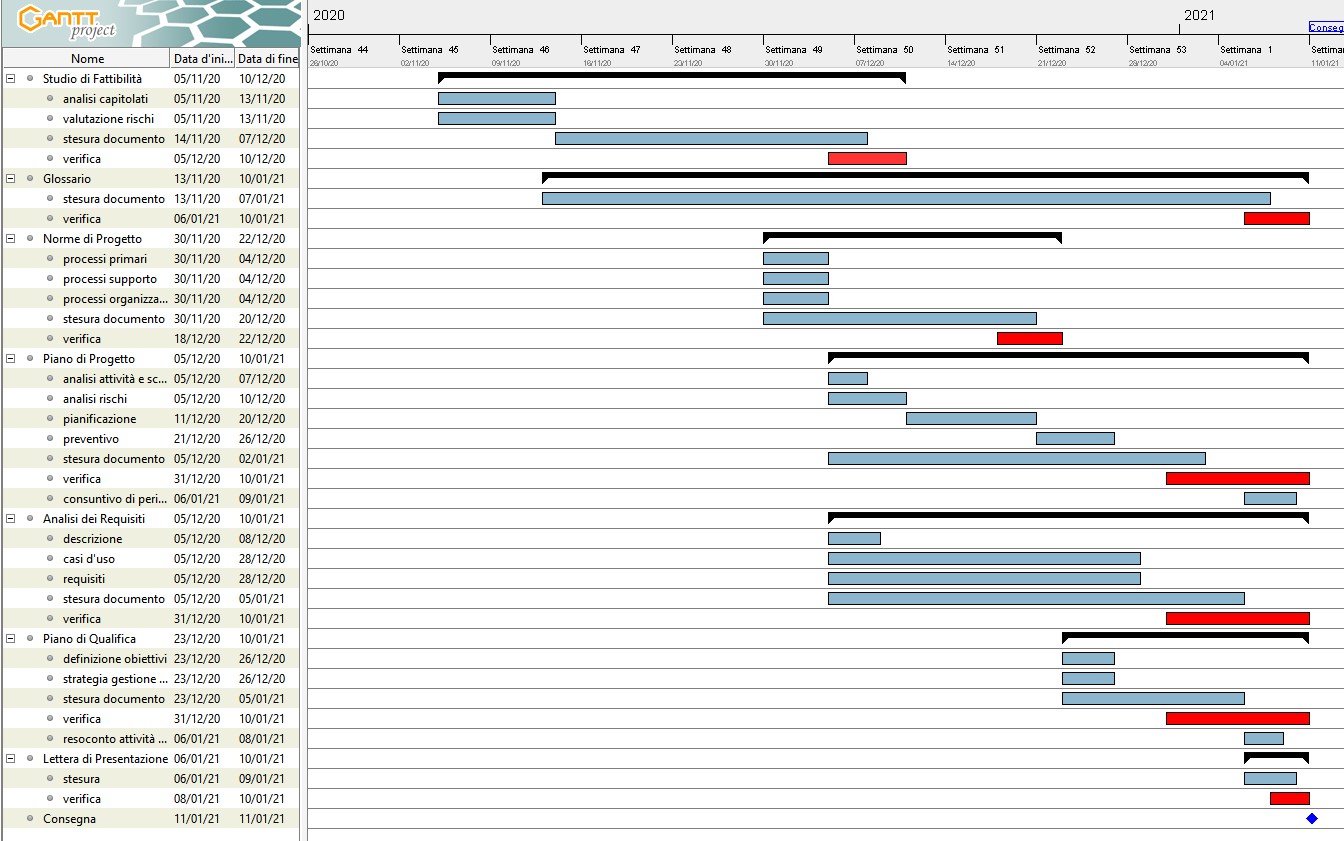
\includegraphics[scale=0.45]{Images/GanttPianificazioneAnalisi.PNG}
	\caption{Diagramma di Gantt dell'attività di Progettazione di dettaglio e Codifica}
\end{figure}